\subsection{Kiến trúc 3 lớp}
\label{sec:three-layer-architecture}

Hệ thống quản lý kí túc xá được chia thành ba tầng với trách nhiệm rõ ràng: lớp
giao diện, lớp nghiệp vụ và lớp dữ liệu. Mô hình này giúp giảm sự phụ thuộc giữa
giao diện, xử lý logic và lưu trữ, từ đó làm cho hệ thống dễ kiểm thử, dễ bảo trì
và dễ mở rộng hơn. Trong dự án ký túc xá, kiến trúc 3 lớp cũng khớp với cách
phân tích BCE ở mức khái niệm và cách triển khai Express.js ở backend.

\subsubsection{Lớp giao diện}
Đây là nơi người dùng tương tác trực tiếp với hệ thống. Các màn hình
Angular chịu trách nhiệm hiển thị dữ liệu, thu nhận thao tác người dùng và gửi
yêu cầu đến backend thông qua API. Lớp này không xử lý quy tắc nghiệp vụ, mà chỉ
tập trung vào giao diện, trải nghiệm người dùng và việc phản hồi thông tin một
cách rõ ràng, nhất quán.

\begin{itemize}
    \item Ví dụ: \texttt{BookingView}, \texttt{PaymentView}, \texttt{ContractView}, \texttt{CheckoutView}, \texttt{RoomView}.
    \item Nhiệm vụ chính: hiển thị danh sách phòng, form đặt cọc, màn hình thanh toán, thông tin hợp đồng và biểu mẫu trả phòng.
    \item Nguyên tắc: không chứa logic nghiệp vụ và không truy cập dữ liệu trực tiếp.
\end{itemize}

\subsubsection{Lớp nghiệp vụ}
Lớp nghiệp vụ xử lý các quy tắc cốt lõi của hệ thống. Đây là nơi kiểm tra trạng
thái phòng, xác nhận thông tin khách hàng, tính tiền đặt cọc, quản lý hợp đồng,
điều phối quy trình trả phòng và tính toán hoàn tiền. Trong backend, lớp này được
triển khai chủ yếu qua các controller và service để đảm bảo luồng xử lý được tách
biệt khỏi giao diện và dữ liệu.

\begin{itemize}
    \item Ví dụ: \texttt{BookingController}, \texttt{PaymentController}, \texttt{ContractController}, \texttt{CheckoutController}, \texttt{RefundCalculator}, \texttt{SchedulerController}.
    \item Nhiệm vụ chính: kiểm tra tính hợp lệ của yêu cầu, cập nhật trạng thái phòng/giường, xử lý đặt cọc, lập hợp đồng và đối soát chi phí.
    \item Nguyên tắc: nhận yêu cầu từ lớp trình bày, làm việc với lớp dữ liệu qua service/repository và không trực tiếp đảm nhiệm giao diện.
\end{itemize}

\subsubsection{Lớp dữ liệu}
Lớp dữ liệu lưu trữ các thực thể và trạng thái bền vững của hệ thống. Các đối
tượng trong lớp này phản ánh trực tiếp dữ liệu nghiệp vụ như khách hàng, nhân
viên, phòng, giường, đặt cọc, thanh toán, hợp đồng và biên bản thanh lý. Ở mức
triển khai, lớp này kết nối với cơ sở dữ liệu Supabase/PostgreSQL thông qua mô
hình dữ liệu và các bảng tương ứng.

\begin{itemize}
    \item Ví dụ: \texttt{Customer}, \texttt{Employee}, \texttt{Room}, \texttt{Bed}, \texttt{DepositRequest}, \texttt{Payment}, \texttt{Contract}, \texttt{CheckoutRequest}, \texttt{Settlement}.
    \item Nhiệm vụ chính: biểu diễn dữ liệu nghiệp vụ, lưu trạng thái và cung cấp cấu trúc cho việc đọc/ghi dữ liệu.
    \item Nguyên tắc: không điều phối luồng xử lý và không chứa logic ra quyết định phức tạp.
\end{itemize}


\begin{figure}[H]
    \centering
    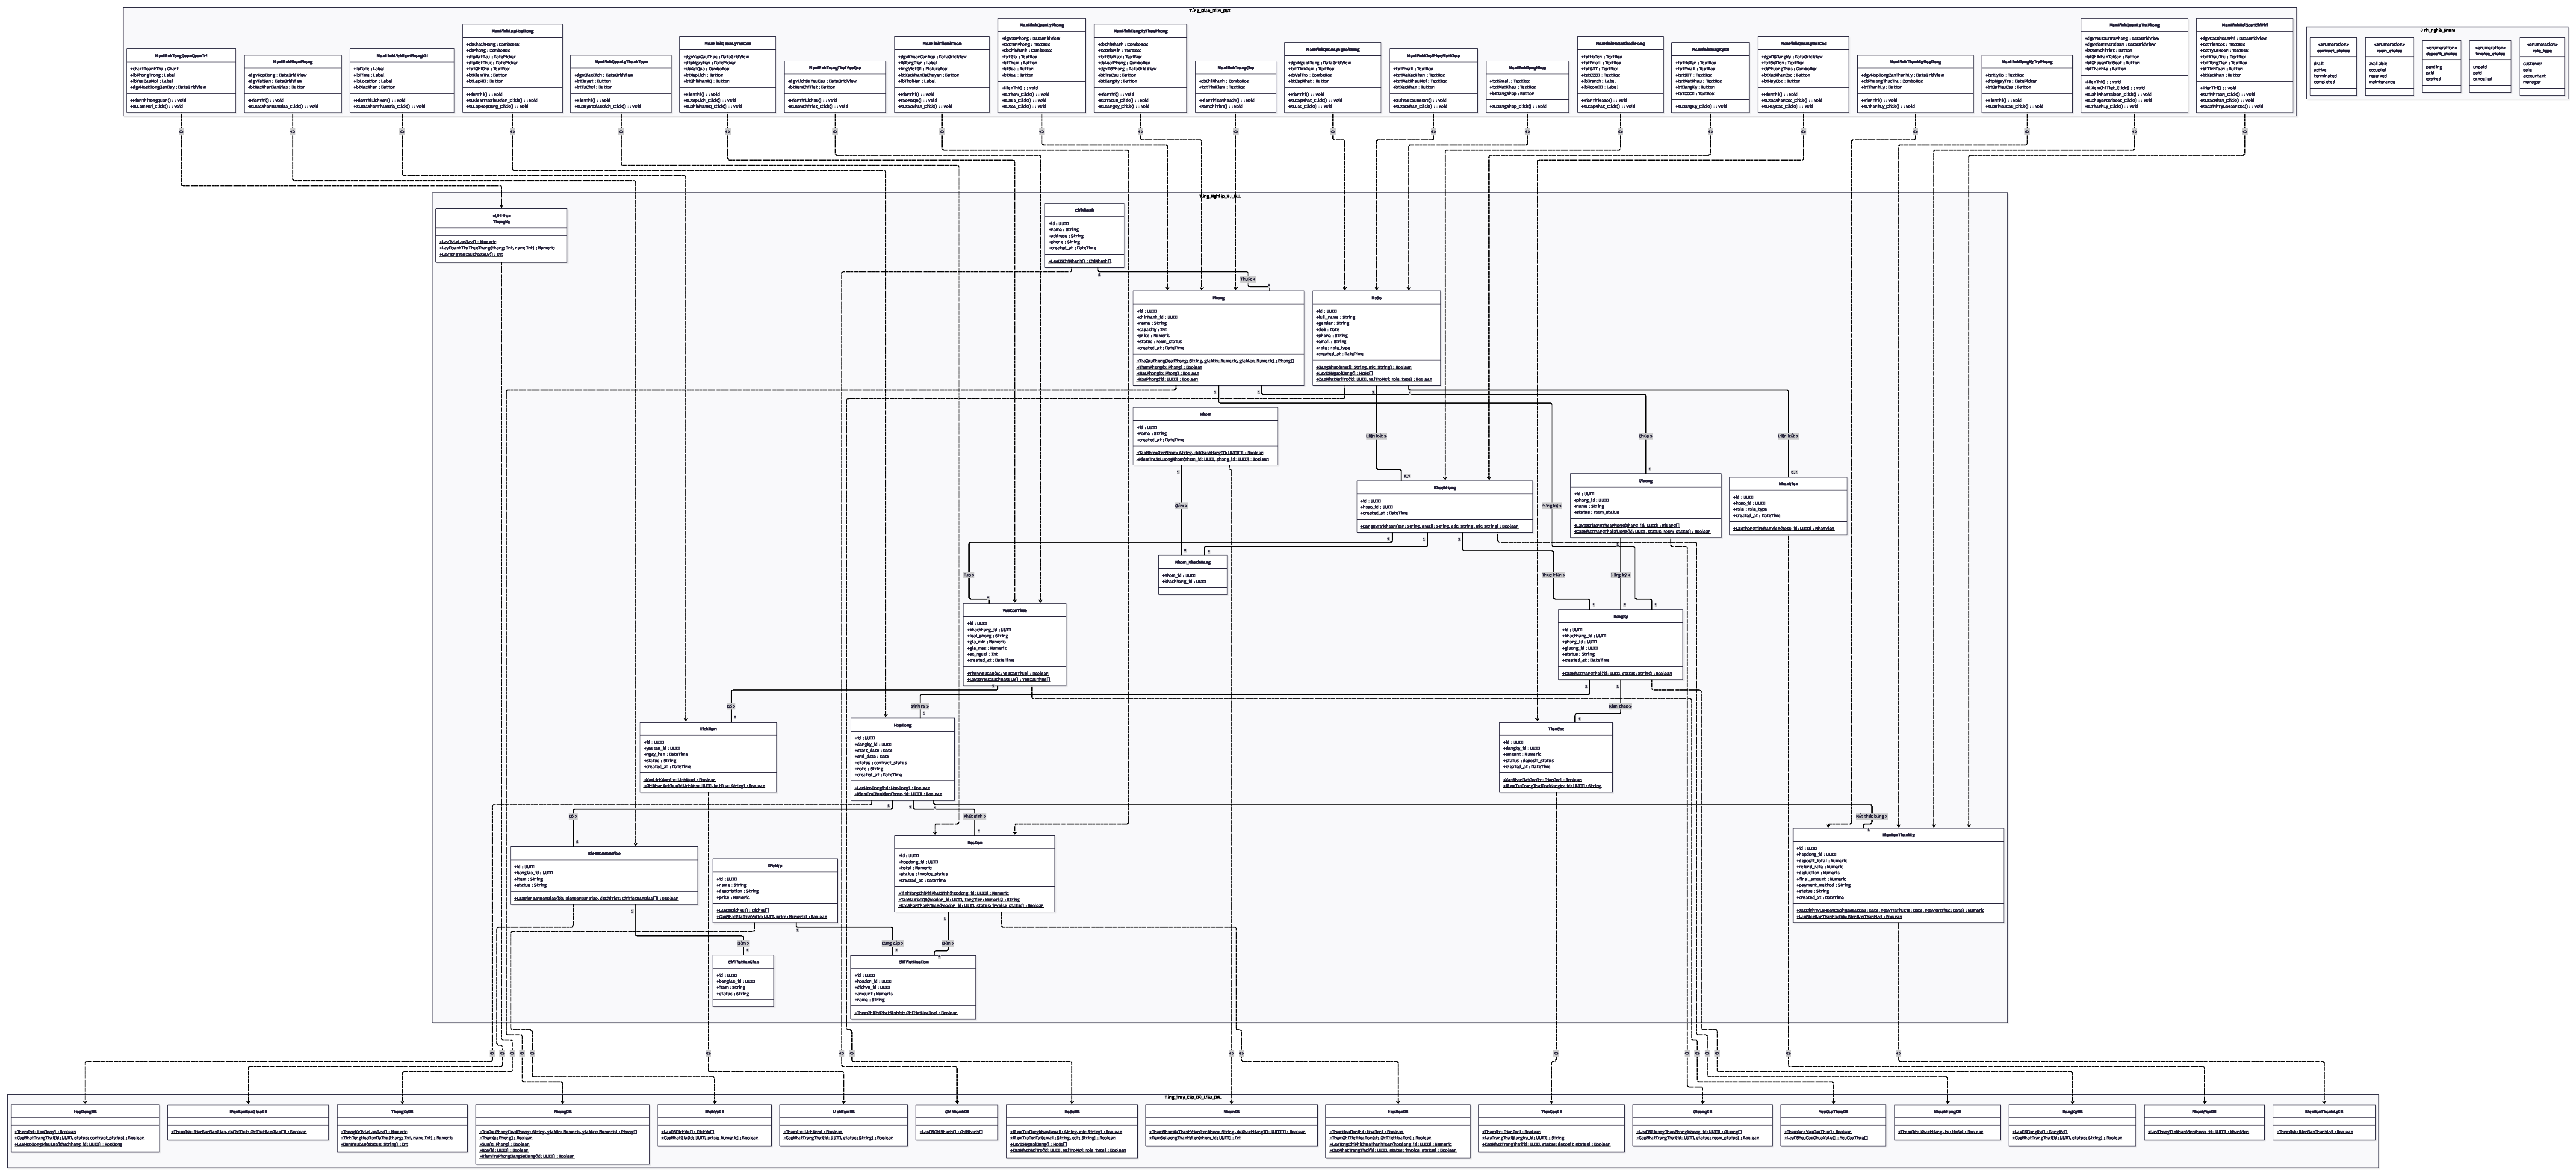
\includegraphics[width=0.98\textwidth]{images/3-Layer.pdf}
    \caption{Sơ đồ điều hướng màn hình hệ thống HomeStay Dorm}
\end{figure}


